O Transmissor/Receptor Assíncrono Universal (\emph{Universal Asynchronous Receiver/Transmitter}, UART), é um periférico de transmissão e recepção de dados usado na comunicação entre dispositivos, sendo esta comunicação realizada de forma serial e assíncrona, ou seja sem a necessidade de transmissão do sinal de clock de referência. Este modo de transmissão faz necessário o uso de apenas duas vias de comunicação uma para a transmissão e outra para a recepção de dados.

\subsection{Padrão da Comunicação}

\begin{figure}[H]
\centering
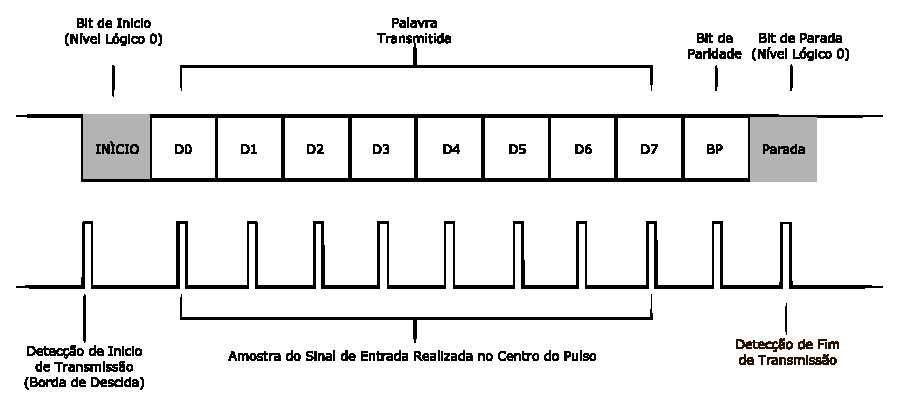
\includegraphics[width=1\textwidth] {figuras/uart.eps}
    \caption{Protocolo de envio na comunicação UART}
    \label{fig:uart}
\end{figure}

Para que a comunicação UART seja realizada é necessário que o sinal de transmissão obedeça a um protocolo. Quando uma palavra é transmitida, primeiro é enviado um bit de início de transmissão para o receptor. Este bit deve ser de nível logico 0 para que a ocorrência da borda de descida sinalize ao receptor que sincronize a amostragem do sinal a ser lido de modo que ela ocorra no meio de cada período de transmissão.  Após transmitir os dados é necessário enviar um bit informando a existência de paridade ou não, e por último é enviado um bit de nível lógico alto para informar o fim da transmissão. Esta sintaxe pode ser observada na figura \ref{fig:uart}.

\subsection{UART do TM4C1294NCPDT}


O Tiva TM4C1294NCPDT possui 4 dispositivos de comunicação UART. 


\section{Na TivaWare}

